\documentclass[11pt]{scrartcl}

\usepackage[top=2cm]{geometry}
\usepackage{url}
\usepackage{tikz}

\title{
  \textbf{\large Database Management and Tuning -- Assignment 7}\\
  Transaction Chopping
}

\author{
 Group Name A3\\
 \large Platzer Hugo, 1421579 \\
 \large Strohmeier Mario, 1422959
}

\begin{document}

\maketitle

{\it Notes:}

\begin{itemize}
\item The chopping graphs may also be drawn by hand and attached as a
  hard copy on paper. In the case of drawings on paper, you need to
  hand in the drawings during the lab.
\item The chopping graphs need to show all S- and C-edges, and you
  need to cross out (or otherwise mark) the S-edges that must be
  removed to get a correct chopping. Also show the write list for each
  chopping graph.
\end{itemize}

\section*{Task 1:  Bank Accounts}

\subsection*{(a) SQL Queries}

{\it Give the SQL queries (including pseudo code if necessary) for each
transaction.}

\paragraph{Transaction T1}

{\small
\begin{verbatim}
...
\end{verbatim}
}

\paragraph{Transaction T2}

{\small
\begin{verbatim}
...
\end{verbatim}
}

\paragraph{Transaction T3}

{\small
\begin{verbatim}
...
\end{verbatim}
}

\subsection*{(b) Model Transactions}

{\it Model all transactions with read/write operations.}

\smallskip

{\it Note: Define the data items first, for example, $a_1$ is
   account\,1, $b_1$ is branch\,1, etc. Define the minimum number of
  data items that represent all possible conflicts in the scenario.}

\begin{enumerate}
\item[T1:]
\item[T2:]
\item[T3:] 
\end{enumerate}

\subsection*{(c) Chopping Graph}

{\it Show the chopping graph and give the finest possible correct
  chopping.}

\medskip

\noindent
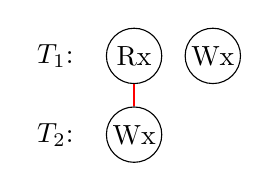
\begin{tikzpicture}[every node/.style={draw,circle,minimum size=2em,inner sep=1}]
\node[draw=none] (T1) at (0, 0) {$T_1$:};
\node (T1_1) at (1, 0) {Rx};
\node (T1_2) at (2, 0) {Wx};
\node[draw=none] (T2) at (0, -1) {$T_2$:};
\node (T2_1) at (1, -1) {Wx};

\draw[draw=red,line width=1pt] (T1_1) -- (T2_1);
\end{tikzpicture}

\medskip

\noindent Finest correct chopping:
\begin{enumerate}
\item[T1:]
\item[T2:]
\item[T3:] 
\end{enumerate}

\subsection*{(d) Two Transactions Update the Same Account}

{\it How does the chopping change if two concurrent transactions of type
$T_1$ can update the same account? Explain.}

\subsection*{(e) Order of Atomic Operations}

{\it The order of the atomic operations in $T_3$ has an impact on the
  chopping. Show two semantically equivalent implementations of $T_3$,
  one which favors chopping, the other which does not favor
  chopping. Explain.}


\section*{Task 2: Chopping Graphs}

\subsection*{(a) All Transactions}

\medskip

[...chopping graph...]

\medskip

\noindent Finest correct chopping:
\begin{enumerate}
\item[T1:]
\item[T2:]
\item[T3:] 
\item[T4:]
\item[T5:]
\item[T6:] 
\end{enumerate}


\subsection*{(b) All Transactions Except T4}

\medskip

[...chopping graph...]

\medskip

\noindent Finest correct chopping:
\begin{enumerate}
\item[T1:]
\item[T2:]
\item[T3:] 
\item[T5:]
\item[T6:] 
\end{enumerate}


\subsection*{Time Spent on this Assignment}

Time in hours: {\bf XXX}

% \bigskip

% \begin{center}
%   \begin{tabular}{c}
%     \hline
%     {\bf Important:} Reference your information sources!
%     \\\hline
%   \end{tabular}
% \end{center}

\end{document}
